% =====================================================================
%  MiniVPN -- Computer Networks Lab Project Report
%  Compile:  pdflatex cn-report.tex   (run twice for contents/references)
%  Needs jiit-logo.png in the same folder.
% =====================================================================
\documentclass[12pt,a4paper]{report}

\usepackage[margin=1in]{geometry}
\usepackage{graphicx}
\usepackage{amsmath}
\usepackage{setspace}
\usepackage{enumitem}
\usepackage{booktabs}
\usepackage{tabularx}
\usepackage{longtable}
\usepackage{float}
\usepackage{xcolor}
\usepackage{listings}
\usepackage{tikz}
\usetikzlibrary{positioning,arrows.meta,shapes.geometric,fit,calc}
\usepackage[hidelinks]{hyperref}

\setstretch{1.3}
\setlist{itemsep=2pt,topsep=4pt}

% Running header and page number (no extra package needed).
% Chapter opening pages keep the plain style (page number only).
\makeatletter
\def\ps@project{%
  \def\@oddhead{\small MiniVPN -- CN Lab Project Report\hfill JIIT, Noida}%
  \let\@evenhead\@oddhead
  \def\@oddfoot{\hfil\thepage\hfil}%
  \let\@evenfoot\@oddfoot}
\makeatother
\pagestyle{project}

\definecolor{codebg}{RGB}{247,247,247}
\definecolor{codekw}{RGB}{0,0,160}
\definecolor{codecm}{RGB}{0,120,0}
\definecolor{codestr}{RGB}{160,30,30}
\lstset{
  language=C, basicstyle=\ttfamily\small, backgroundcolor=\color{codebg},
  keywordstyle=\color{codekw}\bfseries, commentstyle=\color{codecm}\itshape,
  stringstyle=\color{codestr}, frame=single, rulecolor=\color{black!25},
  breaklines=true, columns=fullflexible, numbers=left, numberstyle=\tiny\color{gray},
  xleftmargin=1.5em, framexleftmargin=1.5em, showstringspaces=false, tabsize=4,
  captionpos=b}

% ---------------------------------------------------------------------
%  Front-page details -- edit here
% ---------------------------------------------------------------------
\newcommand{\projecttitle}{MiniVPN: Design and Implementation of a Secure Layer-3 Tunnelling Protocol over UDP}
\newcommand{\doctype}{Computer Networks Lab Project Report}
\newcommand{\semester}{Semester 5}

\begin{document}

% =========================== FRONT PAGE ==============================
\begin{titlepage}
\centering
{\Large\bfseries BACHELOR OF TECHNOLOGY\par}
\vspace{1.2cm}

\includegraphics[width=4.2cm]{jiit-logo.png}\par
\vspace{0.6cm}
{\large Jaypee Institute of Information Technology, Noida\par}
\vspace{1.4cm}
{\LARGE\bfseries \projecttitle\par}
\vspace{1.2cm}
{\Large \semester\par}
\vspace{0.4cm}
{\Large\bfseries \doctype\par}
\vfill
\begin{minipage}[t]{0.52\textwidth}
\raggedright
{\large\bfseries Made By:}\\[6pt]
Sansriti Mishra \hfill 2401030293\\
Mokshi Mittal \hfill 2401030326\\
Sanvi Dhingra \hfill 2401030312
\end{minipage}%
\hfill
\begin{minipage}[t]{0.38\textwidth}
\raggedleft
{\large\bfseries Submitted To:}\\[6pt]
Dr. Anuja Shukla\\
Dr. Kirti Agarwal
\end{minipage}
\vspace{1.5cm}

{\large Department of Computer Science \& Engineering and IT\par}
\end{titlepage}

% ======================== PRELIMINARY PAGES ==========================
\pagenumbering{roman}

\chapter*{Declaration}
\addcontentsline{toc}{chapter}{Declaration}
We hereby declare that the project titled \textbf{``\projecttitle''}, submitted as
part of the Computer Networks Lab in Semester 5 of the Bachelor of Technology programme
at Jaypee Institute of Information Technology, Noida, is our own work. It has not been
submitted elsewhere for any other degree or course. All sources used have been
acknowledged in the references.

\vspace{2cm}
\noindent
\begin{tabular}{@{}ll@{}}
Sansriti Mishra & 2401030293\\[4pt]
Mokshi Mittal & 2401030326\\[4pt]
Sanvi Dhingra & 2401030312
\end{tabular}

\vspace{1cm}
\noindent Date: \rule{4cm}{0.4pt}

\chapter*{Acknowledgement}
\addcontentsline{toc}{chapter}{Acknowledgement}
We thank our faculty, \textbf{Dr. Anuja Shukla} and \textbf{Dr. Kirti Agarwal}, for
their guidance throughout the Computer Networks Lab. Their teaching on the TCP/IP
protocol suite, addressing and routing, transport protocols and network security gave
us the foundation on which this project is built. We also thank the Department of
Computer Science \& Engineering and IT, JIIT Noida, for providing the facilities and
environment to carry out this work.

\chapter*{Abstract}
\addcontentsline{toc}{chapter}{Abstract}
This report presents \textbf{MiniVPN}, a layer-3 virtual private network designed and
implemented from scratch in C. MiniVPN connects devices on different networks into one
private IPv4 subnet (10.8.0.0/24) across the public Internet. IP packets are
encapsulated in UDP datagrams using a custom binary wire protocol.

The protocol begins with a one-round-trip authenticated handshake (HELLO / WELCOME)
that uses X25519 key exchange and HKDF to derive fresh per-direction session keys.
Data packets are protected with ChaCha20-Poly1305 authenticated encryption, a
1024-packet anti-replay window and source-address anti-spoofing. The server assigns
each device a fixed tunnel address, forwards packets between devices, and provides
Internet access through NAT. The client can redirect all of a device's traffic using
longest-prefix routing (\texttt{0.0.0.0/1} and \texttt{128.0.0.0/1}). Because UDP is
unreliable and connectionless, the protocol adds its own retransmission with
exponential backoff, keepalives that hold NAT mappings open, dead-peer detection and
roaming when a device changes networks. A tunnel MTU of 1400 bytes avoids
fragmentation on standard 1500-byte paths.

The system was verified with 53 end-to-end checks across four virtual hosts built with
Linux network namespaces, including packet captures that confirm no plaintext crosses
the wire, an 8 MiB transfer verified by SHA-256, MTU and full-tunnel tests. It reaches
a throughput of about 680 Mbit/s on a laptop.

\tableofcontents
\listoffigures
\listoftables

\clearpage
\pagenumbering{arabic}

% ============================ CHAPTERS ===============================

\chapter{Introduction}

\section{Background}
A \emph{Virtual Private Network} (VPN) creates a private network on top of a public
one. Packets travelling between members of the VPN are \emph{encapsulated} inside other
packets, encrypted and authenticated, then carried across the Internet. To
applications, remote machines appear to be on the same local network.

VPNs are used by companies to give remote employees access to internal services, to
join branch-office networks, and to protect traffic on untrusted Wi-Fi. Well-known
protocols include IPsec, OpenVPN and WireGuard.

\section{Motivation}
A VPN touches almost every layer of the TCP/IP model. Building one requires:
\begin{itemize}
  \item understanding how IP packets are structured, addressed and routed (network layer);
  \item choosing and extending a transport protocol (UDP) and adding reliability where needed;
  \item handling MTU limits so that encapsulated packets do not fragment;
  \item working through Network Address Translation, which almost every home and mobile network uses;
  \item designing a secure protocol: key exchange, authentication, encryption and replay protection;
  \item serving a management interface over HTTP (application layer).
\end{itemize}
Designing our own wire protocol and implementing it end to end turns these textbook
topics into packets that can be captured, inspected and measured.

\section{Problem Statement}
Design and implement a secure VPN protocol and system that connects multiple devices
across the Internet into one private IPv4 network. It must carry arbitrary IP traffic
transparently, resist eavesdropping, tampering, replay and spoofing, work through NAT,
and recover from packet loss and network changes.

\section{Objectives}
\begin{enumerate}
  \item Design an IP-in-UDP encapsulation protocol with a precise byte-level packet format.
  \item Implement an authenticated one-round-trip handshake that derives fresh session keys.
  \item Protect data with authenticated encryption, an anti-replay window and anti-spoofing.
  \item Assign addresses from a tunnel subnet and route packets between devices and to the Internet through NAT.
  \item Choose an MTU that prevents fragmentation of tunnelled packets.
  \item Add reliability on top of UDP: retransmission with backoff, keepalives, timeouts and roaming.
  \item Support a full-tunnel mode using longest-prefix routing.
  \item Verify behaviour with packet captures and end-to-end tests on a virtual multi-host network.
\end{enumerate}

\section{Organisation of the Report}
Chapter~\ref{ch:background} reviews the networking background. Chapter~\ref{ch:design}
describes the architecture, addressing plan and wire protocol. Chapter~\ref{ch:impl}
explains how each networking mechanism is implemented. Chapter~\ref{ch:testing}
presents testing and results, and Chapter~\ref{ch:conclusion} concludes with
limitations and future work.

% ---------------------------------------------------------------------
\chapter{Background and Related Work}\label{ch:background}

\section{Layering and Tunnelling}
In the TCP/IP model each layer adds its own header to the data from the layer above.
\emph{Tunnelling} breaks the usual order: a complete network-layer packet becomes the
\emph{payload} of another protocol. In MiniVPN an inner IPv4 packet (addressed within
10.8.0.0/24) is carried inside a UDP datagram, which is carried inside an outer IPv4
packet addressed between the devices' real public addresses.

\begin{figure}[H]
\centering
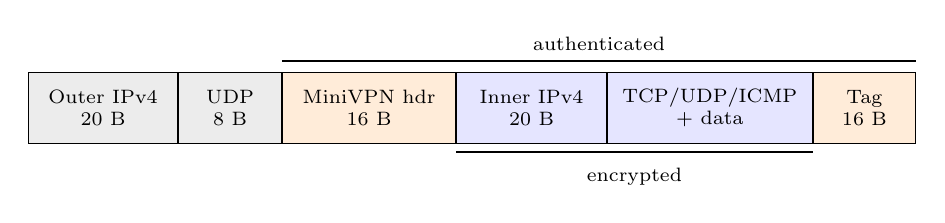
\begin{tikzpicture}[f/.style={draw,minimum height=0.9cm,font=\scriptsize,align=center}]
  \node[f,fill=gray!15,minimum width=1.9cm] (a) {Outer IPv4\\20 B};
  \node[f,fill=gray!15,minimum width=1.3cm,right=0pt of a] (b) {UDP\\8 B};
  \node[f,fill=orange!15,minimum width=2.2cm,right=0pt of b] (c) {MiniVPN hdr\\16 B};
  \node[f,fill=blue!10,minimum width=1.9cm,right=0pt of c] (d) {Inner IPv4\\20 B};
  \node[f,fill=blue!10,minimum width=2.6cm,right=0pt of d] (e) {TCP/UDP/ICMP\\+ data};
  \node[f,fill=orange!15,minimum width=1.3cm,right=0pt of e] (t) {Tag\\16 B};
  \draw[thick] ([yshift=-3pt]d.south west) -- ([yshift=-3pt]e.south east)
       node[midway,below=2pt,font=\scriptsize]{encrypted};
  \draw[thick] ([yshift=4pt]c.north west) -- ([yshift=4pt]t.north east)
       node[midway,above,font=\scriptsize]{authenticated};
\end{tikzpicture}
\caption{Packet encapsulation in MiniVPN}
\label{fig:encap}
\end{figure}

\section{Virtual Network Interfaces}
To capture the packets that applications send, MiniVPN uses a Linux \textbf{TUN}
interface. A TUN interface is a network-layer device with no hardware behind it: the
kernel routes packets to it like any interface, but they are delivered to a user
program instead of a wire. Packets the program writes back appear to the kernel as if
they had arrived on that interface. (A TAP interface is the layer-2 equivalent that
carries Ethernet frames.)

\section{Why UDP and not TCP}
VPNs that run over TCP suffer from \emph{TCP-over-TCP meltdown}. When a packet is lost,
both the inner TCP connection and the outer tunnel TCP connection back off and
retransmit, and their timers interfere, causing large delays. UDP adds only 8 bytes of
header and no reliability of its own. Lost tunnel packets are simply recovered by the
inner protocol (for example the application's own TCP connection), just as on a normal
network. MiniVPN only adds reliability where it needs it: for its own handshake.

\section{Network Address Translation}
Most devices sit behind NAT routers that rewrite private source addresses
(e.g.\ 192.168.1.10) to a public address and port. NAT keeps a mapping only while
traffic flows; idle UDP mappings expire, often in 30 seconds or less. A VPN must
therefore (a) start the conversation from the client side, (b) send periodic
keepalives, and (c) accept that the client's apparent public IP:port may change
(\emph{NAT rebinding}).

\section{Cryptographic Building Blocks}
\begin{description}[style=nextline]
  \item[X25519 (RFC 7748)] Elliptic-curve Diffie--Hellman key exchange. Both sides compute the same shared secret from exchanged public keys.
  \item[HKDF-SHA256 (RFC 5869)] Derives several independent keys from one shared secret.
  \item[HMAC-SHA256 (RFC 2104)] A keyed message authentication code, used to authenticate handshake messages.
  \item[ChaCha20-Poly1305 (RFC 8439)] Authenticated encryption with associated data (AEAD). Encrypts the payload and produces a 16-byte tag that detects any modification.
  \item[Ed25519 (RFC 8032)] A digital signature scheme, used to sign license files.
\end{description}

\section{Existing VPN Protocols}
\begin{table}[H]
\centering
\caption{Comparison with existing VPN protocols}
\begin{tabularx}{\textwidth}{@{}lXXX@{}}
\toprule
 & \textbf{IPsec (ESP)} & \textbf{OpenVPN} & \textbf{MiniVPN}\\
\midrule
Layer & Network (IP protocol 50) & Application, over UDP/TCP & Application, over UDP\\
Key exchange & IKEv2 (multi-message) & TLS handshake & 1 round trip, X25519\\
NAT traversal & Needs NAT-T (UDP 4500) & Yes & Yes (UDP, keepalives)\\
Roaming & Needs MOBIKE & Limited & Yes\\
Replay protection & Sliding window & Sliding window & 1024-packet window\\
Configuration & Complex & Certificates (PKI) & One file per device\\
\bottomrule
\end{tabularx}
\end{table}
MiniVPN is closest in design to WireGuard: a small, fixed set of modern algorithms,
UDP transport, one-round-trip handshake and roaming. Our protocol differs in its
handshake (a pre-shared device key plus ephemeral X25519), its message formats and
its server-side device registry with live revocation.

% ---------------------------------------------------------------------
\chapter{System Design}\label{ch:design}

\section{Architecture}

\begin{figure}[H]
\centering
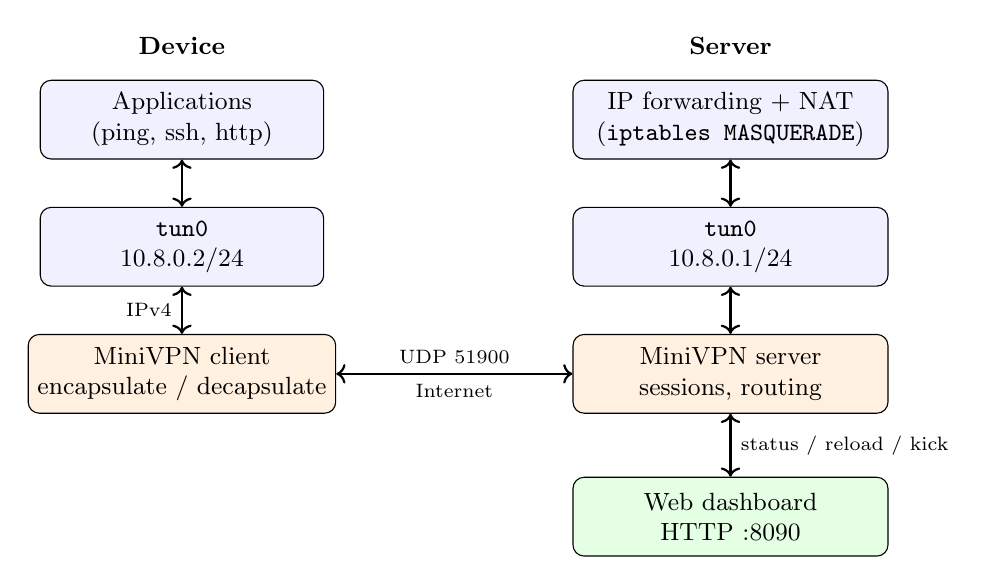
\begin{tikzpicture}[
  box/.style={draw,rounded corners,align=center,minimum height=1cm,font=\small,fill=blue!6},
  arr/.style={-{Stealth},thick}]
  \node[box,minimum width=3.6cm] (app) {Applications\\(ping, ssh, http)};
  \node[box,below=0.6cm of app,minimum width=3.6cm] (tun) {\texttt{tun0}\\10.8.0.2/24};
  \node[box,below=0.6cm of tun,minimum width=3.6cm,fill=orange!12] (cli) {MiniVPN client\\encapsulate / decapsulate};
  \node[box,right=3.0cm of cli,minimum width=4cm,fill=orange!12] (srv) {MiniVPN server\\sessions, routing};
  \node[box,above=0.6cm of srv,minimum width=4cm] (stun) {\texttt{tun0}\\10.8.0.1/24};
  \node[box,above=0.6cm of stun,minimum width=4cm] (lan) {IP forwarding + NAT\\(\texttt{iptables MASQUERADE})};
  \node[box,below=0.8cm of srv,minimum width=4cm,fill=green!10] (adm) {Web dashboard\\HTTP :8090};
  \draw[arr,<->] (app) -- (tun);
  \draw[arr,<->] (tun) -- node[left,font=\scriptsize]{IPv4} (cli);
  \draw[arr,<->] (cli) -- node[above,font=\scriptsize]{UDP 51900}
                          node[below,font=\scriptsize]{Internet} (srv);
  \draw[arr,<->] (srv) -- (stun);
  \draw[arr,<->] (stun) -- (lan);
  \draw[arr,<->] (adm) -- node[right,font=\scriptsize]{status / reload / kick} (srv);
  \node[font=\small\bfseries,above=0.2cm of app] {Device};
  \node[font=\small\bfseries,above=0.2cm of lan] {Server};
\end{tikzpicture}
\caption{MiniVPN architecture}
\label{fig:arch}
\end{figure}

The system follows a hub-and-spoke (star) topology. Every device keeps one UDP session
with the central server. The server decrypts each packet and decides where it goes:
another device (re-encrypted with that device's keys), a service on the server itself,
or the Internet through NAT. An HTTP dashboard shows connected devices, their public
endpoints and live traffic, and lets an administrator disable or revoke a device.

\section{Addressing Plan}
\begin{table}[H]
\centering
\caption{Default addressing}
\begin{tabular}{@{}ll@{}}
\toprule
\textbf{Item} & \textbf{Value}\\
\midrule
Tunnel subnet & 10.8.0.0/24 (netmask 255.255.255.0)\\
Network address & 10.8.0.0 (not assigned)\\
Server tunnel address & 10.8.0.1\\
Device addresses & 10.8.0.2 -- 10.8.0.254 (fixed per device)\\
Broadcast address & 10.8.0.255 (not assigned)\\
Transport & UDP, server port 51900\\
\bottomrule
\end{tabular}
\end{table}
Each device keeps the same tunnel address across reconnections, so other devices and
firewall rules can refer to it reliably. The server uses an array indexed by host
number (address minus network address) to find the session for a destination address
in constant time.

\section{Packet Flow}
\begin{enumerate}
  \item An application on device A (10.8.0.2) sends a packet to device B (10.8.0.3).
        The kernel's routing table matches 10.8.0.0/24 on \texttt{tun0}.
  \item The MiniVPN client reads the IPv4 packet from \texttt{tun0}, encrypts it with its
        client-to-server key and sends it to the server's public IP on UDP port 51900.
  \item The server finds the session by its 32-bit session id, checks the replay window and
        verifies the authentication tag.
  \item The server parses the inner IPv4 header. If the source is not 10.8.0.2, the packet
        is dropped (anti-spoofing).
  \item The destination 10.8.0.3 belongs to device B, so the server re-encrypts the packet
        with B's server-to-client key and sends it to B's current public endpoint.
  \item B decrypts the packet and writes it into its \texttt{tun0}; B's kernel delivers it
        to the application.
\end{enumerate}
If the destination is not a VPN device, the server writes the packet to its own
\texttt{tun0}, and the kernel forwards it (with NAT for Internet destinations).

\section{Wire Protocol}
All integers are in network byte order (big-endian). There are five message types.

\subsection{Device identity and keys}
Each device has a public 16-byte \emph{device id} and a secret 32-byte \emph{device key}.
Keys are derived as:
\[
\begin{aligned}
\textit{auth\_key} &= \mathrm{HKDF}(\textit{device\_key},\ \text{``minivpn v2 handshake auth''})\\
k_{c2s} \,\|\, k_{s2c} &= \mathrm{HKDF}(\text{salt}=\textit{device\_key},\ \text{ikm}=\mathrm{X25519}(e_c, E_s),\ \text{info}=\ldots)
\end{aligned}
\]
An attacker needs both the device key and an ephemeral private key to read a session.
Ephemeral keys are wiped after the handshake, giving \emph{forward secrecy}: a device
key stolen later cannot decrypt recorded traffic.

\subsection{Handshake}
\begin{figure}[H]
\centering
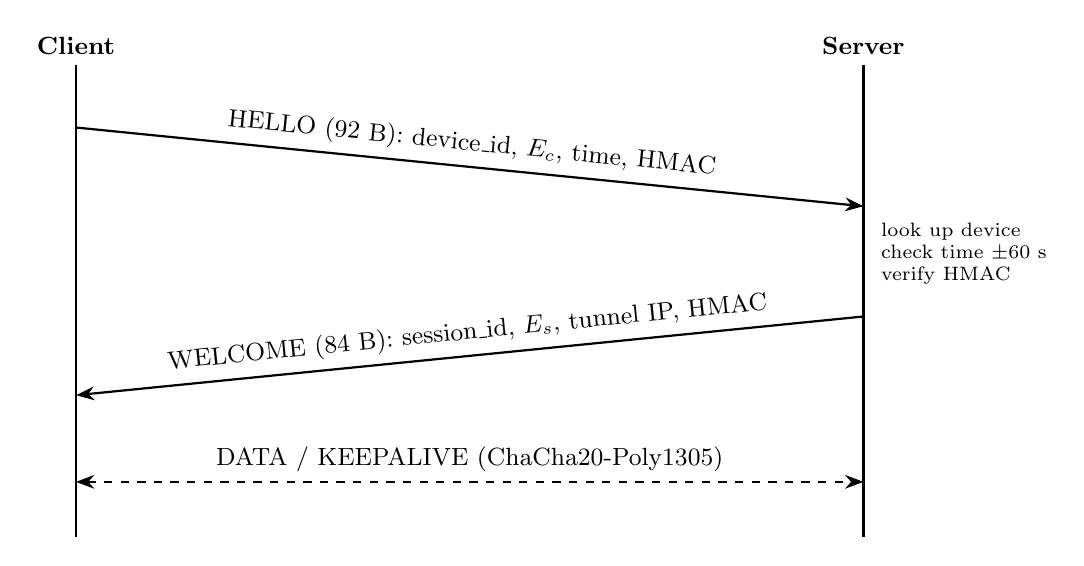
\begin{tikzpicture}[font=\small]
  \draw[thick] (0,0) node[above]{\textbf{Client}} -- (0,-6);
  \draw[thick] (10,0) node[above]{\textbf{Server}} -- (10,-6);
  \draw[-{Stealth},thick] (0,-0.8) -- node[above,sloped]{HELLO (92 B): device\_id, $E_c$, time, HMAC} (10,-1.8);
  \node[right,align=left,font=\scriptsize] at (10.1,-2.4) {look up device\\check time $\pm$60 s\\verify HMAC};
  \draw[-{Stealth},thick] (10,-3.2) -- node[above,sloped]{WELCOME (84 B): session\_id, $E_s$, tunnel IP, HMAC} (0,-4.2);
  \draw[{Stealth}-{Stealth},thick,dashed] (0,-5.3) -- node[above]{DATA / KEEPALIVE (ChaCha20-Poly1305)} (10,-5.3);
\end{tikzpicture}
\caption{One-round-trip handshake}
\label{fig:handshake}
\end{figure}

\begin{table}[H]
\centering
\caption{HELLO and WELCOME message formats}
\begin{tabular}{@{}rlrl@{}}
\toprule
\multicolumn{2}{c}{\textbf{HELLO} (client $\to$ server, 92 B)} & \multicolumn{2}{c}{\textbf{WELCOME} (server $\to$ client, 84 B)}\\
\textbf{Off.} & \textbf{Field} & \textbf{Off.} & \textbf{Field}\\
\midrule
0 & type = 1 & 0 & type = 2\\
1 & version = 2 & 1 & version = 2\\
2 & reserved (2) & 2 & tunnel MTU (2)\\
4 & device id (16) & 4 & session id (4)\\
20 & client X25519 public key (32) & 8 & server X25519 public key (32)\\
52 & Unix time (8) & 40 & client tunnel IP (4)\\
60 & HMAC over bytes 0--59 (32) & 44 & netmask (4)\\
 & & 48 & server tunnel IP (4)\\
 & & 52 & HMAC over HELLO MAC + bytes 0--51 (32)\\
\bottomrule
\end{tabular}
\end{table}

\begin{itemize}
  \item The WELCOME carries the network configuration (address, netmask, MTU), so the
        client needs no separate address-assignment protocol such as DHCP.
  \item An unknown or disabled device, or a bad MAC, gets \textbf{no reply}, so port
        scanners cannot tell that a VPN server is listening.
  \item The timestamp must be within $\pm60$\,s, which limits replay of old HELLOs.
  \item The WELCOME MAC covers the HELLO's MAC, binding the answer to that exact request.
  \item A retransmitted HELLO (same ephemeral key) gets the cached WELCOME again, so a
        lost WELCOME never creates a duplicate session.
\end{itemize}

\subsection{Data packets}
\begin{table}[H]
\centering
\caption{Data packet format}
\begin{tabular}{@{}lll@{}}
\toprule
\textbf{Offset} & \textbf{Size} & \textbf{Field}\\
\midrule
0 & 1 & type: 3 DATA, 4 KEEPALIVE, 5 DISCONNECT\\
1 & 3 & reserved\\
4 & 4 & session id\\
8 & 8 & counter (also the nonce)\\
16 & $n$ & ChaCha20-Poly1305 ciphertext (the inner IPv4 packet)\\
$16+n$ & 16 & authentication tag\\
\bottomrule
\end{tabular}
\end{table}
The 16-byte header is authenticated as associated data but not encrypted, so the
receiver can find the session before decrypting. Each direction uses its own key, so
a nonce is never reused under the same key.

\subsection{Timers}
\begin{table}[H]
\centering
\caption{Protocol timers}
\begin{tabular}{@{}ll@{}}
\toprule
\textbf{Event} & \textbf{Value}\\
\midrule
Keepalive after idle & 10 s (both sides)\\
Client: server considered dead & 30 s without receiving\\
Server: session expires & 60 s without receiving\\
HELLO retransmission & 1, 2, 4, 8, 8, \ldots\ s (exponential backoff, capped)\\
Fresh ephemeral key for HELLO & after 45 s of retrying\\
Rekey & every 300 s\\
\bottomrule
\end{tabular}
\end{table}

% ---------------------------------------------------------------------
\chapter{Implementation}\label{ch:impl}
This chapter describes how each networking mechanism is implemented. Code excerpts
are taken directly from the source.

\section{Capturing Packets with a TUN Interface}
The daemon opens \texttt{/dev/net/tun} and creates a TUN interface with the flag
\texttt{IFF\_NO\_PI}, so each \texttt{read()} returns exactly one raw IPv4 packet. It then
assigns the interface its address, netmask and MTU. From this point the kernel routes
all 10.8.0.0/24 traffic into the VPN.

\begin{lstlisting}[caption={Creating the TUN interface (\texttt{src/tun.c})}]
int fd = open("/dev/net/tun", O_RDWR | O_NONBLOCK | O_CLOEXEC);
struct ifreq ifr;
memset(&ifr, 0, sizeof ifr);
ifr.ifr_flags = IFF_TUN | IFF_NO_PI;     /* layer 3, no extra header */
snprintf(ifr.ifr_name, IFNAMSIZ, "%s", name);
ioctl(fd, TUNSETIFF, &ifr);
/* then: SIOCSIFADDR, SIOCSIFNETMASK, SIOCSIFMTU, SIOCSIFFLAGS (up) */
\end{lstlisting}

\section{IPv4 Header Processing and Forwarding}
After decrypting a packet, the server reads three fields from the inner IPv4 header:
the version (high 4 bits of byte 0), the total length (bytes 2--3) and the source and
destination addresses (bytes 12--15 and 16--19).

\begin{lstlisting}[caption={Validating, anti-spoofing and routing a packet (\texttt{src/server.c})}]
static void route_from_client(server *s, session *x, const uint8_t *pkt, size_t len)
{
    if (len < 20 || (pkt[0] >> 4) != 4)        /* IPv4 only */
        return;
    size_t total = get_u16(pkt + 2);            /* total length */
    if (total < 20 || total > len)
        return;

    uint32_t src = get_u32(pkt + 12);
    uint32_t dst = get_u32(pkt + 16);
    if (src != x->vip) {                        /* anti-spoofing */
        s->dropped++;
        return;
    }

    session *target = find_by_ip(s, dst);
    if (target) {                               /* device to device */
        send_sealed(s, target, PKT_DATA, pkt, total);
        return;
    }
    write(s->tun, pkt, total);                  /* to the kernel */
}
\end{lstlisting}

\paragraph{Anti-spoofing.} A device is only allowed to send packets whose source
address is its own tunnel address. Without this check, one authenticated device could
impersonate another inside the VPN. This is the same idea as ingress filtering
(RFC 2827) on the public Internet.

\paragraph{Using the total-length field.} The length from the IPv4 header, not the
number of bytes received, decides how much is forwarded. This rejects truncated
packets and ignores any padding.

\section{MTU and Fragmentation}
Every tunnelled packet grows by 60 bytes: 20 (outer IPv4) + 8 (UDP) + 16 (MiniVPN
header) + 16 (authentication tag). If the tunnel interface also used an MTU of 1500,
full-size packets would become 1560 bytes and would need to be fragmented on the
physical path, which hurts performance and is often blocked.

\[
1400 \text{ (tunnel MTU)} + 60 \text{ (overhead)} = 1460 \le 1500 \text{ (Ethernet MTU)}
\]

MiniVPN sets the tunnel MTU to 1400 and sends it to the client in the WELCOME message,
leaving 40 bytes of headroom for paths with extra headers (for example PPPoE). Packets
larger than the tunnel MTU with the Don't-Fragment bit set are refused locally by the
kernel, which triggers Path MTU Discovery in the sender's TCP.

\section{Routing}

\subsection{Server-side forwarding and NAT}
For devices to reach the Internet through the VPN, the server enables IP forwarding
and masquerades the tunnel subnet behind its public interface:

\begin{lstlisting}[language=bash,caption={Enabling forwarding and NAT (\texttt{scripts/server-nat.sh})}]
sysctl -qw net.ipv4.ip_forward=1
iptables -t nat -A POSTROUTING -s 10.8.0.0/24 -o "$UPLINK" -j MASQUERADE
iptables -A FORWARD -s 10.8.0.0/24 -o "$UPLINK" -j ACCEPT
iptables -A FORWARD -d 10.8.0.0/24 -i "$UPLINK" \
         -m conntrack --ctstate RELATED,ESTABLISHED -j ACCEPT
\end{lstlisting}
\texttt{MASQUERADE} rewrites the source address of outgoing packets to the server's
public address. The connection-tracking rule lets only replies to connections started
from inside the VPN back in.

\subsection{Full-tunnel mode and longest-prefix match}
In full-tunnel mode, all of a device's Internet traffic goes through the VPN. The naive
approach, replacing the default route, breaks the tunnel itself: the encrypted UDP
packets to the server would also be routed into the tunnel. MiniVPN uses three routes
instead:

\begin{table}[H]
\centering
\caption{Client routing table in full-tunnel mode}
\begin{tabular}{@{}lll@{}}
\toprule
\textbf{Destination} & \textbf{Via} & \textbf{Purpose}\\
\midrule
\textit{server-ip}/32 & original gateway & keeps the tunnel's own UDP traffic on the real link\\
0.0.0.0/1 & \texttt{tun0} & first half of the IPv4 address space\\
128.0.0.0/1 & \texttt{tun0} & second half of the IPv4 address space\\
0.0.0.0/0 & original gateway & original default route, left untouched\\
\bottomrule
\end{tabular}
\end{table}
Routers choose the \emph{most specific} (longest-prefix) matching route. The two /1
routes together cover every address and are more specific than /0, so they win. The
/32 host route to the server is more specific still. When the VPN stops, the three
routes are removed and the original default route is in effect again, unchanged.

\begin{lstlisting}[caption={Full-tunnel routes (\texttt{src/client.c})}]
/* pin a host route to the server via the old gateway, then add 0/1 and
 * 128/1 which are more specific than the existing default route */
route_add(server, 0xffffffffu, c->orig_gw, c->orig_dev);
route_add(0x00000000u, 0x80000000u, 0, c->dev);
route_add(0x80000000u, 0x80000000u, 0, c->dev);
\end{lstlisting}

\section{Reliability over UDP}
UDP gives no delivery guarantee, so MiniVPN adds reliability only where it is needed.

\begin{itemize}
  \item \textbf{Handshake retransmission.} If no WELCOME arrives, the client resends HELLO
        after 1, 2, 4, 8, 8, \ldots\ seconds. Exponential backoff avoids flooding a server
        that is down or a congested link. After 45 seconds a fresh ephemeral key is used.
  \item \textbf{Idempotent server.} A repeated HELLO with the same key gets the cached
        WELCOME, so a lost WELCOME is recovered without a second session.
  \item \textbf{Data packets are not retransmitted.} Inner protocols (TCP) already recover
        lost data end to end; retransmitting in the tunnel would cause TCP-over-TCP problems.
  \item \textbf{Keepalives and dead-peer detection.} After 10 s of silence each side sends
        an empty encrypted KEEPALIVE. A client that hears nothing for 30 s starts a new
        handshake; the server deletes sessions idle for 60 s.
\end{itemize}

\section{NAT Traversal and Roaming}
Because the client always sends first, its NAT router creates a mapping that lets the
server's replies through. The 10-second keepalives refresh this mapping before it
expires. If the client's public address changes (Wi-Fi to mobile data, or the NAT
assigns a new port), the server notices on the next \emph{authenticated} packet and
updates the session's endpoint:

\begin{lstlisting}[caption={Roaming (\texttt{src/server.c})}]
ssize_t n = channel_open(&x->ch, pkt, len, &type, plain);
if (n < 0)
    return;   /* bad tag or replay: never move the session */

/* Authenticated traffic from a new address: the client roamed (Wi-Fi to
 * mobile, NAT rebinding). Follow it. */
if (x->peer.sin_addr.s_addr != from->sin_addr.s_addr ||
    x->peer.sin_port != from->sin_port)
    x->peer = *from;
\end{lstlisting}
Updating only after the tag is verified means an attacker cannot redirect a session by
sending forged packets from another address.

\section{Anti-Replay Window}
An attacker could record a valid encrypted packet and send it again later. Each packet
carries a 64-bit counter. The receiver keeps a 1024-bit sliding bitmap of recently seen
counters, the same technique used by IPsec ESP (RFC 4303). Since UDP may reorder
packets, slightly older counters are still accepted if not seen before.

\begin{lstlisting}[caption={Replay check (\texttt{src/replay.c})}]
int replay_check(const replay_window *w, uint64_t ctr)
{
    if (!w->seen_any || ctr > w->top)
        return 0;                      /* newer than anything seen */
    if (w->top - ctr >= REPLAY_WINDOW)
        return -1;                     /* too old */
    return bit_get(w, ctr) ? -1 : 0;   /* duplicate? */
}
\end{lstlisting}
The window advances only \emph{after} the authentication tag has been verified, so
forged packets cannot push it forward and cause valid packets to be dropped.

\section{Application Layer: Web Dashboard}
The management dashboard is an HTTP server on port 8090 (Python standard library). It
lists devices with their tunnel address, online state, current public endpoint
(IP:port) and bytes sent and received, and offers disable, enable, revoke and kick
actions. It is protected by:
\begin{itemize}
  \item salted password hashing and login lockout after repeated failures;
  \item session cookies marked \texttt{HttpOnly} and \texttt{SameSite};
  \item CSRF tokens and \texttt{Origin} checks on every state-changing request;
  \item optional TLS (HTTPS) for access from other machines.
\end{itemize}
The dashboard talks to the running VPN server over a local socket with three commands:
\texttt{status}, \texttt{reload} and \texttt{kick}, so changes apply without a restart.

% ---------------------------------------------------------------------
\chapter{Testing and Results}\label{ch:testing}

\section{Virtual Test Network}
A realistic test needs several hosts on separate networks. Linux \emph{network
namespaces} give each process its own interfaces, addresses and routing table, so one
computer can simulate several machines. Virtual Ethernet (\texttt{veth}) pairs act as
cables between them. The integration test builds the following topology:

\begin{figure}[H]
\centering
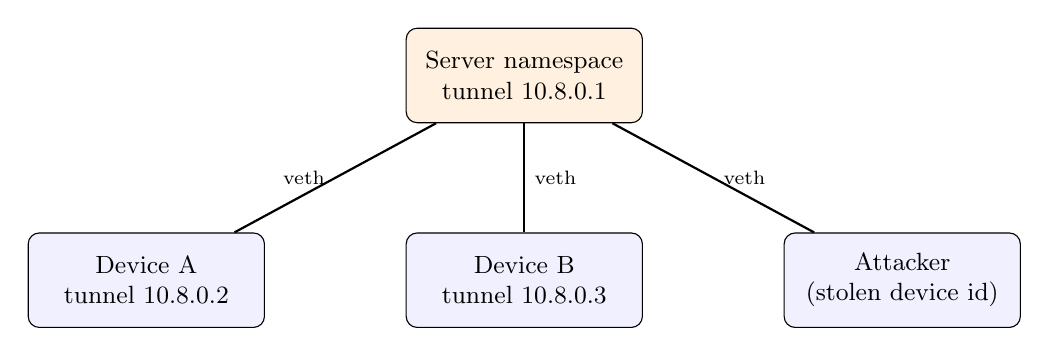
\begin{tikzpicture}[ns/.style={draw,rounded corners,minimum width=3cm,minimum height=1.2cm,align=center,font=\small,fill=blue!6}]
  \node[ns,fill=orange!12] (s) at (0,0) {Server namespace\\tunnel 10.8.0.1};
  \node[ns] (a) at (-4.8,-2.6) {Device A\\tunnel 10.8.0.2};
  \node[ns] (b) at (0,-2.6) {Device B\\tunnel 10.8.0.3};
  \node[ns] (c) at (4.8,-2.6) {Attacker\\(stolen device id)};
  \draw[thick] (s) -- node[left,font=\scriptsize]{veth} (a);
  \draw[thick] (s) -- node[right,font=\scriptsize]{veth} (b);
  \draw[thick] (s) -- node[right,font=\scriptsize]{veth} (c);
\end{tikzpicture}
\caption{Integration test topology}
\end{figure}

\section{Test Suites}
\begin{table}[H]
\centering
\caption{Test suites}
\begin{tabularx}{\textwidth}{@{}lrX@{}}
\toprule
\textbf{Suite} & \textbf{Checks} & \textbf{Coverage}\\
\midrule
Protocol unit tests & 119 & Crypto against RFC 4231, 5869, 7748 and 8032 test vectors; packet tampering; replay window; handshake binding; message parsing\\
Dashboard tests & 13 & Login, password hashing, CSRF, origin checks, lockout, device limits\\
End-to-end tests & 53 & Across 4 network namespaces (below)\\
\bottomrule
\end{tabularx}
\end{table}

\section{End-to-End Test Scenarios}
\begin{longtable}{@{}p{5.5cm}p{9cm}@{}}
\caption{Selected end-to-end checks}\\
\toprule
\textbf{Scenario} & \textbf{Expected and observed result}\\
\midrule
\endfirsthead
\toprule
\textbf{Scenario} & \textbf{Expected and observed result}\\
\midrule
\endhead
Connectivity & Devices ping the server (10.8.0.1) and each other through the tunnel\\
Address assignment & Each device receives its fixed address and netmask in the WELCOME\\
Wrong key / unknown device & HELLO gets no reply; no session is created\\
Encrypted wire & \texttt{tcpdump} on the physical link sees only UDP to port 51900 with no plaintext payload\\
Bulk transfer & 8 MiB file served over HTTP between devices; SHA-256 matches at both ends\\
MTU & 1372-byte ping with DF set (1400-byte IP packet) passes unfragmented; a 1428-byte DF packet is refused locally\\
Kick, disable, enable, revoke & Each takes effect on the live server; traffic stops or resumes immediately\\
Rekey & New session keys installed while traffic continues\\
Server restart & Clients detect the dead peer and reconnect automatically\\
Full tunnel & All traffic routed via \texttt{tun0} using the \texttt{0/1} + \texttt{128/1} routes; server still reachable\\
\bottomrule
\end{longtable}
All 119 unit checks, 13 dashboard tests and 53 end-to-end checks pass.

\section{Packet Capture Analysis}
Capturing on the physical interface during a ping shows that an observer sees only:
\begin{itemize}
  \item the outer IPv4 header (public addresses of device and server);
  \item the UDP header (source port and destination port 51900);
  \item the 16-byte MiniVPN header (type, session id, counter);
  \item ciphertext and tag, indistinguishable from random bytes.
\end{itemize}
The inner addresses (10.8.0.x), the protocol (ICMP, TCP) and the payload are hidden.
Modifying any byte of a captured packet and re-sending it causes the receiver to drop
it because the tag no longer verifies; re-sending it unmodified is dropped by the
replay window.

% Add Wireshark screenshots here, for example:
% \begin{figure}[H]
%   \centering
%   \includegraphics[width=\textwidth]{wireshark.png}
%   \caption{Wireshark capture of tunnelled traffic}
% \end{figure}

\section{Performance}
Measured on a laptop, MiniVPN reaches approximately \textbf{680 Mbit/s} through the
encrypted tunnel. The protocol overhead per packet is 60 bytes; for full-size 1400-byte
packets this is about $60/1460 \approx 4.1\%$ of the bytes on the wire.

\section{Sample Output}
\begin{lstlisting}[language={},numbers=none,basicstyle=\ttfamily\scriptsize,caption={Device list with public endpoints and traffic}]
$ sudo minivpn-admin list
NAME           TUNNEL IP   STATUS  ONLINE  CONNECTED FROM       RECEIVED     SENT
alice-laptop   10.8.0.2    active  yes     49.36.112.7:55120      1.7 GB  394.9 MB
build-server   10.8.0.4    active  yes     34.93.10.4:51900      11.8 GB    8.5 GB
carol-phone    10.8.0.5    active  -       -                          -         -
\end{lstlisting}
The \texttt{CONNECTED FROM} column shows each device's public IP:port as seen by the
server, i.e.\ after any NAT on the device's side.

% ---------------------------------------------------------------------
\chapter{Conclusion and Future Work}\label{ch:conclusion}

\section{Conclusion}
MiniVPN is a complete, working layer-3 VPN with its own wire protocol, written from
scratch in C. It applies the main topics of computer networks end to end:
encapsulation across layers, IPv4 header processing, subnetting and address
assignment, routing with longest-prefix match, MTU sizing, NAT, transport over UDP with
selective reliability, and secure protocol design with authenticated key exchange,
AEAD, replay protection and forward secrecy. Testing on a virtual multi-host network
and analysis of packet captures confirmed that traffic is carried correctly and
remains confidential and tamper-proof on the wire.

\section{Limitations}
\begin{itemize}
  \item Only IPv4 is carried inside the tunnel.
  \item Hub-and-spoke only: device-to-device traffic always passes through the server.
  \item Clients run on Linux only.
  \item The protocol has not been independently security-audited.
\end{itemize}

\section{Future Work}
\begin{itemize}
  \item IPv6 inside the tunnel and IPv6 transport.
  \item Peer-to-peer paths between devices using UDP hole punching, with the server as fallback relay.
  \item Path MTU probing to choose the tunnel MTU automatically.
  \item Windows and macOS clients.
  \item Batched packet I/O (\texttt{sendmmsg}/\texttt{recvmmsg}) and multiple cores for higher throughput.
\end{itemize}

% ---------------------------------------------------------------------
\renewcommand{\bibname}{References}
\begin{thebibliography}{99}
\addcontentsline{toc}{chapter}{References}
\bibitem{tanenbaum} A. S. Tanenbaum, D. J. Wetherall, \emph{Computer Networks}, 5th ed., Pearson, 2011.
\bibitem{kurose} J. F. Kurose, K. W. Ross, \emph{Computer Networking: A Top-Down Approach}, 8th ed., Pearson, 2021.
\bibitem{rfc791} J. Postel, \emph{Internet Protocol}, RFC 791, 1981.
\bibitem{rfc768} J. Postel, \emph{User Datagram Protocol}, RFC 768, 1980.
\bibitem{rfc1191} J. Mogul, S. Deering, \emph{Path MTU Discovery}, RFC 1191, 1990.
\bibitem{rfc3022} P. Srisuresh, K. Egevang, \emph{Traditional IP Network Address Translator (Traditional NAT)}, RFC 3022, 2001.
\bibitem{rfc2827} P. Ferguson, D. Senie, \emph{Network Ingress Filtering}, RFC 2827, 2000.
\bibitem{rfc4303} S. Kent, \emph{IP Encapsulating Security Payload (ESP)}, RFC 4303, 2005.
\bibitem{wg} J. A. Donenfeld, ``WireGuard: Next Generation Kernel Network Tunnel,'' in \emph{Proc. NDSS}, 2017.
\bibitem{rfc8439} Y. Nir, A. Langley, \emph{ChaCha20 and Poly1305 for IETF Protocols}, RFC 8439, 2018.
\bibitem{rfc7748} A. Langley, M. Hamburg, S. Turner, \emph{Elliptic Curves for Security}, RFC 7748, 2016.
\bibitem{rfc5869} H. Krawczyk, P. Eronen, \emph{HMAC-based Extract-and-Expand Key Derivation Function (HKDF)}, RFC 5869, 2010.
\bibitem{tuntap} Linux kernel documentation, \emph{Universal TUN/TAP device driver}, \url{https://docs.kernel.org/networking/tuntap.html}.
\end{thebibliography}

% ---------------------------------------------------------------------
\appendix
\chapter{Build and Run Instructions}
\begin{lstlisting}[language=bash,numbers=none,caption={Quick demo on Linux or WSL2}]
sudo apt install build-essential libssl-dev python3
make
sudo ./scripts/demo.sh        # dashboard at http://localhost:8090
sudo make integration         # end-to-end tests
\end{lstlisting}

\begin{lstlisting}[language=bash,numbers=none,caption={Server and one device}]
sudo minivpn-admin init --endpoint vpn.example.com
sudo minivpn-admin add laptop -o laptop.conf
sudo ./scripts/server-nat.sh up            # forwarding + NAT
sudo minivpn server --config /etc/minivpn/server.conf
# on the device:
sudo minivpn client --config laptop.conf   # add -g for full tunnel
\end{lstlisting}

\begin{lstlisting}[language=bash,numbers=none,caption={Observing the tunnel}]
sudo tcpdump -ni eth0 udp port 51900       # encrypted outer packets
sudo tcpdump -ni tun0                      # plaintext inner packets
ip route                                   # 0/1 and 128/1 in full-tunnel mode
\end{lstlisting}

\end{document}
